\documentclass[twoside]{book}

% Packages required by doxygen
\usepackage{fixltx2e}
\usepackage{calc}
\usepackage{doxygen}
\usepackage[export]{adjustbox} % also loads graphicx
\usepackage{graphicx}
\usepackage[utf8]{inputenc}
\usepackage{makeidx}
\usepackage{multicol}
\usepackage{multirow}
\PassOptionsToPackage{warn}{textcomp}
\usepackage{textcomp}
\usepackage[nointegrals]{wasysym}
\usepackage[table]{xcolor}

% Font selection
\usepackage[T1]{fontenc}
\usepackage[scaled=.90]{helvet}
\usepackage{courier}
\usepackage{amssymb}
\usepackage{sectsty}
\renewcommand{\familydefault}{\sfdefault}
\allsectionsfont{%
  \fontseries{bc}\selectfont%
  \color{darkgray}%
}
\renewcommand{\DoxyLabelFont}{%
  \fontseries{bc}\selectfont%
  \color{darkgray}%
}
\newcommand{\+}{\discretionary{\mbox{\scriptsize$\hookleftarrow$}}{}{}}

% Page & text layout
\usepackage{geometry}
\geometry{%
  a4paper,%
  top=2.5cm,%
  bottom=2.5cm,%
  left=2.5cm,%
  right=2.5cm%
}
\tolerance=750
\hfuzz=15pt
\hbadness=750
\setlength{\emergencystretch}{15pt}
\setlength{\parindent}{0cm}
\setlength{\parskip}{0.2cm}
\makeatletter
\renewcommand{\paragraph}{%
  \@startsection{paragraph}{4}{0ex}{-1.0ex}{1.0ex}{%
    \normalfont\normalsize\bfseries\SS@parafont%
  }%
}
\renewcommand{\subparagraph}{%
  \@startsection{subparagraph}{5}{0ex}{-1.0ex}{1.0ex}{%
    \normalfont\normalsize\bfseries\SS@subparafont%
  }%
}
\makeatother

% Headers & footers
\usepackage{fancyhdr}
\pagestyle{fancyplain}
\fancyhead[LE]{\fancyplain{}{\bfseries\thepage}}
\fancyhead[CE]{\fancyplain{}{}}
\fancyhead[RE]{\fancyplain{}{\bfseries\leftmark}}
\fancyhead[LO]{\fancyplain{}{\bfseries\rightmark}}
\fancyhead[CO]{\fancyplain{}{}}
\fancyhead[RO]{\fancyplain{}{\bfseries\thepage}}
\fancyfoot[LE]{\fancyplain{}{}}
\fancyfoot[CE]{\fancyplain{}{}}
\fancyfoot[RE]{\fancyplain{}{\bfseries\scriptsize Generated on Mon Jun 13 2016 16\+:25\+:25 for Tokenizer by Doxygen }}
\fancyfoot[LO]{\fancyplain{}{\bfseries\scriptsize Generated on Mon Jun 13 2016 16\+:25\+:25 for Tokenizer by Doxygen }}
\fancyfoot[CO]{\fancyplain{}{}}
\fancyfoot[RO]{\fancyplain{}{}}
\renewcommand{\footrulewidth}{0.4pt}
\renewcommand{\chaptermark}[1]{%
  \markboth{#1}{}%
}
\renewcommand{\sectionmark}[1]{%
  \markright{\thesection\ #1}%
}

% Indices & bibliography
\usepackage{natbib}
\usepackage[titles]{tocloft}
\setcounter{tocdepth}{3}
\setcounter{secnumdepth}{5}
\makeindex

% Hyperlinks (required, but should be loaded last)
\usepackage{ifpdf}
\ifpdf
  \usepackage[pdftex,pagebackref=true]{hyperref}
\else
  \usepackage[ps2pdf,pagebackref=true]{hyperref}
\fi
\hypersetup{%
  colorlinks=true,%
  linkcolor=blue,%
  citecolor=blue,%
  unicode%
}

% Custom commands
\newcommand{\clearemptydoublepage}{%
  \newpage{\pagestyle{empty}\cleardoublepage}%
}


%===== C O N T E N T S =====

\begin{document}

% Titlepage & ToC
\hypersetup{pageanchor=false,
             bookmarks=true,
             bookmarksnumbered=true,
             pdfencoding=unicode
            }
\pagenumbering{roman}
\begin{titlepage}
\vspace*{7cm}
\begin{center}%
{\Large Tokenizer }\\
\vspace*{1cm}
{\large Generated by Doxygen 1.8.10}\\
\vspace*{0.5cm}
{\small Mon Jun 13 2016 16:25:25}\\
\end{center}
\end{titlepage}
\clearemptydoublepage
\tableofcontents
\clearemptydoublepage
\pagenumbering{arabic}
\hypersetup{pageanchor=true}

%--- Begin generated contents ---
\chapter{Hierarchical Index}
\section{Class Hierarchy}
This inheritance list is sorted roughly, but not completely, alphabetically\+:\begin{DoxyCompactList}
\item \contentsline{section}{tokenizer.\+tokenizer.\+App}{\pageref{classtokenizer_1_1tokenizer_1_1_app}}{}
\item \contentsline{section}{tokenizer.\+tokenizer.\+Check\+Empty}{\pageref{classtokenizer_1_1tokenizer_1_1_check_empty}}{}
\item \contentsline{section}{tokenizer.\+tokenizer.\+File\+Controller}{\pageref{classtokenizer_1_1tokenizer_1_1_file_controller}}{}
\item \contentsline{section}{tokenizer.\+tokenizer.\+Load\+Files}{\pageref{classtokenizer_1_1tokenizer_1_1_load_files}}{}
\item \contentsline{section}{tokenizer.\+tokenizer.\+Tokenizer\+Main}{\pageref{classtokenizer_1_1tokenizer_1_1_tokenizer_main}}{}
\item J\+Frame\begin{DoxyCompactList}
\item \contentsline{section}{tokenizer.\+tokenizer.\+Frame}{\pageref{classtokenizer_1_1tokenizer_1_1_frame}}{}
\end{DoxyCompactList}
\item J\+Panel\begin{DoxyCompactList}
\item \contentsline{section}{tokenizer.\+tokenizer.\+Panel}{\pageref{classtokenizer_1_1tokenizer_1_1_panel}}{}
\end{DoxyCompactList}
\end{DoxyCompactList}

\chapter{Class Index}
\section{Class List}
Here are the classes, structs, unions and interfaces with brief descriptions\+:\begin{DoxyCompactList}
\item\contentsline{section}{\hyperlink{classtokenizer_1_1tokenizer_1_1_app}{tokenizer.\+tokenizer.\+App} }{\pageref{classtokenizer_1_1tokenizer_1_1_app}}{}
\item\contentsline{section}{\hyperlink{classtokenizer_1_1tokenizer_1_1_check_empty}{tokenizer.\+tokenizer.\+Check\+Empty} }{\pageref{classtokenizer_1_1tokenizer_1_1_check_empty}}{}
\item\contentsline{section}{\hyperlink{classtokenizer_1_1tokenizer_1_1_file_controller}{tokenizer.\+tokenizer.\+File\+Controller} }{\pageref{classtokenizer_1_1tokenizer_1_1_file_controller}}{}
\item\contentsline{section}{\hyperlink{classtokenizer_1_1tokenizer_1_1_frame}{tokenizer.\+tokenizer.\+Frame} }{\pageref{classtokenizer_1_1tokenizer_1_1_frame}}{}
\item\contentsline{section}{\hyperlink{classtokenizer_1_1tokenizer_1_1_load_files}{tokenizer.\+tokenizer.\+Load\+Files} }{\pageref{classtokenizer_1_1tokenizer_1_1_load_files}}{}
\item\contentsline{section}{\hyperlink{classtokenizer_1_1tokenizer_1_1_panel}{tokenizer.\+tokenizer.\+Panel} }{\pageref{classtokenizer_1_1tokenizer_1_1_panel}}{}
\item\contentsline{section}{\hyperlink{classtokenizer_1_1tokenizer_1_1_tokenizer_main}{tokenizer.\+tokenizer.\+Tokenizer\+Main} }{\pageref{classtokenizer_1_1tokenizer_1_1_tokenizer_main}}{}
\end{DoxyCompactList}

\chapter{Class Documentation}
\hypertarget{classtokenizer_1_1tokenizer_1_1_app}{}\section{tokenizer.\+tokenizer.\+App Class Reference}
\label{classtokenizer_1_1tokenizer_1_1_app}\index{tokenizer.\+tokenizer.\+App@{tokenizer.\+tokenizer.\+App}}
\subsection*{Static Public Member Functions}
\begin{DoxyCompactItemize}
\item 
static void \hyperlink{classtokenizer_1_1tokenizer_1_1_app_a25f9e2a083e8c4ab601da2aa1b589475}{main} (String\mbox{[}$\,$\mbox{]} args)
\end{DoxyCompactItemize}


\subsection{Detailed Description}
Clase principal del programa \begin{DoxyAuthor}{Author}
Bianney 
\end{DoxyAuthor}


\subsection{Member Function Documentation}
\hypertarget{classtokenizer_1_1tokenizer_1_1_app_a25f9e2a083e8c4ab601da2aa1b589475}{}\index{tokenizer\+::tokenizer\+::\+App@{tokenizer\+::tokenizer\+::\+App}!main@{main}}
\index{main@{main}!tokenizer\+::tokenizer\+::\+App@{tokenizer\+::tokenizer\+::\+App}}
\subsubsection[{main(\+String[] args)}]{\setlength{\rightskip}{0pt plus 5cm}static void tokenizer.\+tokenizer.\+App.\+main (
\begin{DoxyParamCaption}
\item[{String\mbox{[}$\,$\mbox{]}}]{args}
\end{DoxyParamCaption}
)\hspace{0.3cm}{\ttfamily [static]}}\label{classtokenizer_1_1tokenizer_1_1_app_a25f9e2a083e8c4ab601da2aa1b589475}
Método principal Crea una ventana con las distintas opciones que permite ejecutar el programa 
\begin{DoxyParams}{Parameters}
{\em args} & \\
\hline
\end{DoxyParams}


The documentation for this class was generated from the following file\+:\begin{DoxyCompactItemize}
\item 
src/main/java/tokenizer/tokenizer/App.\+java\end{DoxyCompactItemize}

\hypertarget{classtokenizer_1_1tokenizer_1_1_check_empty}{}\section{tokenizer.\+tokenizer.\+Check\+Empty Class Reference}
\label{classtokenizer_1_1tokenizer_1_1_check_empty}\index{tokenizer.\+tokenizer.\+Check\+Empty@{tokenizer.\+tokenizer.\+Check\+Empty}}
\subsection*{Static Public Member Functions}
\begin{DoxyCompactItemize}
\item 
\hypertarget{classtokenizer_1_1tokenizer_1_1_check_empty_a910efb1028beefb9dcf414d1bbc5a1f5}{}static boolean {\bfseries check} (J\+Combo\+Box$<$ String $>$ input)\label{classtokenizer_1_1tokenizer_1_1_check_empty_a910efb1028beefb9dcf414d1bbc5a1f5}

\end{DoxyCompactItemize}


The documentation for this class was generated from the following file\+:\begin{DoxyCompactItemize}
\item 
src/main/java/tokenizer/tokenizer/Check\+Empty.\+java\end{DoxyCompactItemize}

\hypertarget{classtokenizer_1_1tokenizer_1_1_file_controller}{}\section{tokenizer.\+tokenizer.\+File\+Controller Class Reference}
\label{classtokenizer_1_1tokenizer_1_1_file_controller}\index{tokenizer.\+tokenizer.\+File\+Controller@{tokenizer.\+tokenizer.\+File\+Controller}}
\subsection*{Public Member Functions}
\begin{DoxyCompactItemize}
\item 
\hypertarget{classtokenizer_1_1tokenizer_1_1_file_controller_a390b1263b57bb514699dbf9d11d7c83f}{}void {\bfseries delete\+File} (File file)\label{classtokenizer_1_1tokenizer_1_1_file_controller_a390b1263b57bb514699dbf9d11d7c83f}

\item 
\hypertarget{classtokenizer_1_1tokenizer_1_1_file_controller_a82f8beb57186a72d8f95a7aac8bbd34c}{}void {\bfseries add\+Text} (File input, String text)\label{classtokenizer_1_1tokenizer_1_1_file_controller_a82f8beb57186a72d8f95a7aac8bbd34c}

\item 
\hypertarget{classtokenizer_1_1tokenizer_1_1_file_controller_a6b462a791fe2cfc4754e9f9d084210ff}{}void {\bfseries add} (File output)\label{classtokenizer_1_1tokenizer_1_1_file_controller_a6b462a791fe2cfc4754e9f9d084210ff}

\item 
\hypertarget{classtokenizer_1_1tokenizer_1_1_file_controller_a58d45676902a83d6b319601a134000bd}{}String {\bfseries file\+To\+String} (File input)\label{classtokenizer_1_1tokenizer_1_1_file_controller_a58d45676902a83d6b319601a134000bd}

\end{DoxyCompactItemize}
\subsection*{Static Public Member Functions}
\begin{DoxyCompactItemize}
\item 
\hypertarget{classtokenizer_1_1tokenizer_1_1_file_controller_ac89b0a4919b5d5ea6ce658382ed68a0c}{}static String\mbox{[}$\,$\mbox{]} {\bfseries load} ()\label{classtokenizer_1_1tokenizer_1_1_file_controller_ac89b0a4919b5d5ea6ce658382ed68a0c}

\end{DoxyCompactItemize}
\subsection*{Static Public Attributes}
\begin{DoxyCompactItemize}
\item 
\hypertarget{classtokenizer_1_1tokenizer_1_1_file_controller_a68619eb967ec8d9e8cee9828d0a013a7}{}static String {\bfseries final\+Text} = \char`\"{}\char`\"{}\label{classtokenizer_1_1tokenizer_1_1_file_controller_a68619eb967ec8d9e8cee9828d0a013a7}

\end{DoxyCompactItemize}


The documentation for this class was generated from the following file\+:\begin{DoxyCompactItemize}
\item 
src/main/java/tokenizer/tokenizer/File\+Controller.\+java\end{DoxyCompactItemize}

\hypertarget{classtokenizer_1_1tokenizer_1_1_frame}{}\section{tokenizer.\+tokenizer.\+Frame Class Reference}
\label{classtokenizer_1_1tokenizer_1_1_frame}\index{tokenizer.\+tokenizer.\+Frame@{tokenizer.\+tokenizer.\+Frame}}
Inheritance diagram for tokenizer.\+tokenizer.\+Frame\+:\begin{figure}[H]
\begin{center}
\leavevmode
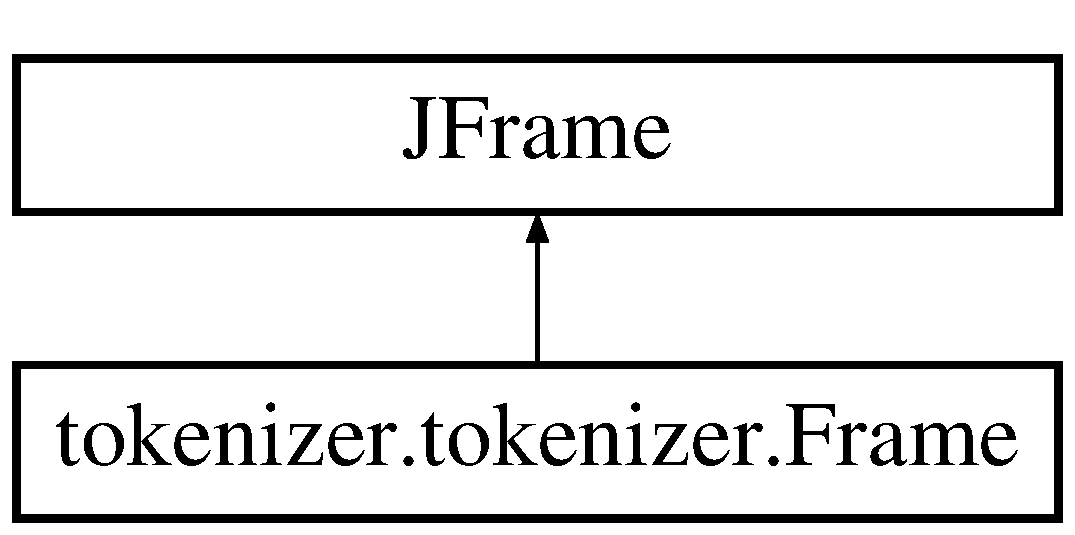
\includegraphics[height=2.000000cm]{classtokenizer_1_1tokenizer_1_1_frame}
\end{center}
\end{figure}
\subsection*{Public Member Functions}
\begin{DoxyCompactItemize}
\item 
\hypertarget{classtokenizer_1_1tokenizer_1_1_frame_ae413453366a008d2250ed120391987c2}{}{\bfseries Frame} (J\+Panel panel, String title)\label{classtokenizer_1_1tokenizer_1_1_frame_ae413453366a008d2250ed120391987c2}

\end{DoxyCompactItemize}


The documentation for this class was generated from the following file\+:\begin{DoxyCompactItemize}
\item 
src/main/java/tokenizer/tokenizer/Frame.\+java\end{DoxyCompactItemize}

\hypertarget{classtokenizer_1_1tokenizer_1_1_load_files}{}\section{tokenizer.\+tokenizer.\+Load\+Files Class Reference}
\label{classtokenizer_1_1tokenizer_1_1_load_files}\index{tokenizer.\+tokenizer.\+Load\+Files@{tokenizer.\+tokenizer.\+Load\+Files}}
\subsection*{Static Public Member Functions}
\begin{DoxyCompactItemize}
\item 
\hypertarget{classtokenizer_1_1tokenizer_1_1_load_files_a6f654927dccf8a90c4288c02e108f472}{}static String\mbox{[}$\,$\mbox{]} {\bfseries load} ()\label{classtokenizer_1_1tokenizer_1_1_load_files_a6f654927dccf8a90c4288c02e108f472}

\end{DoxyCompactItemize}


The documentation for this class was generated from the following file\+:\begin{DoxyCompactItemize}
\item 
src/main/java/tokenizer/tokenizer/Load\+Files.\+java\end{DoxyCompactItemize}

\hypertarget{classtokenizer_1_1tokenizer_1_1_panel}{}\section{tokenizer.\+tokenizer.\+Panel Class Reference}
\label{classtokenizer_1_1tokenizer_1_1_panel}\index{tokenizer.\+tokenizer.\+Panel@{tokenizer.\+tokenizer.\+Panel}}
Inheritance diagram for tokenizer.\+tokenizer.\+Panel\+:\begin{figure}[H]
\begin{center}
\leavevmode
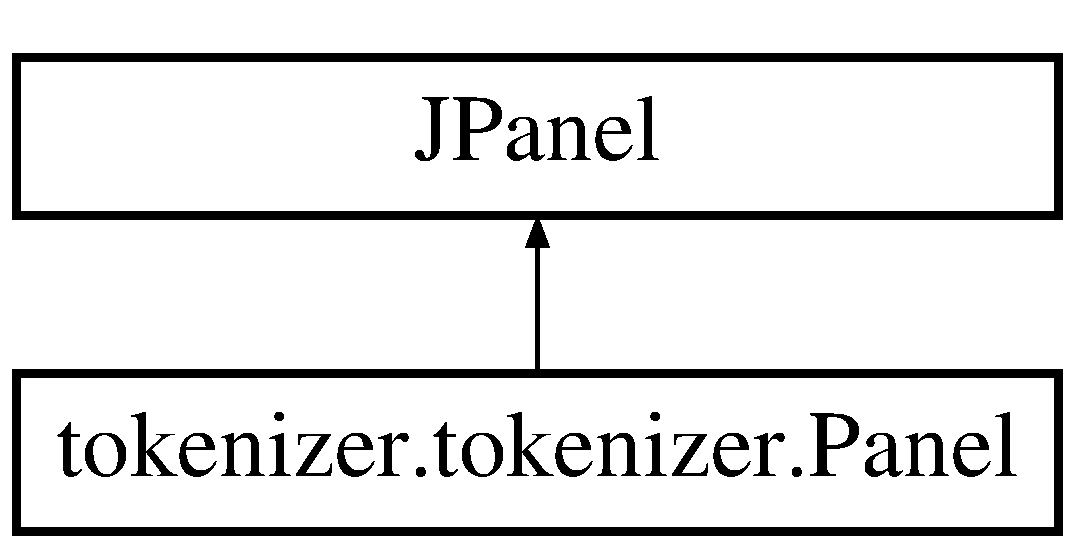
\includegraphics[height=2.000000cm]{classtokenizer_1_1tokenizer_1_1_panel}
\end{center}
\end{figure}
\subsection*{Public Attributes}
\begin{DoxyCompactItemize}
\item 
\hypertarget{classtokenizer_1_1tokenizer_1_1_panel_a02478f6b50abf2c065f425d5a8d1f0a2}{}J\+Button {\bfseries load\+Button} = new J\+Button(load\+File)\label{classtokenizer_1_1tokenizer_1_1_panel_a02478f6b50abf2c065f425d5a8d1f0a2}

\item 
\hypertarget{classtokenizer_1_1tokenizer_1_1_panel_a8d0d8b60a433bacb5033744ab95fd29b}{}J\+Button {\bfseries go\+Button} = new J\+Button(go)\label{classtokenizer_1_1tokenizer_1_1_panel_a8d0d8b60a433bacb5033744ab95fd29b}

\item 
\hypertarget{classtokenizer_1_1tokenizer_1_1_panel_aa295c5f118634fa54028f6209d76403c}{}J\+Button {\bfseries delete\+Button} = new J\+Button(delete)\label{classtokenizer_1_1tokenizer_1_1_panel_aa295c5f118634fa54028f6209d76403c}

\end{DoxyCompactItemize}


The documentation for this class was generated from the following file\+:\begin{DoxyCompactItemize}
\item 
src/main/java/tokenizer/tokenizer/Panel.\+java\end{DoxyCompactItemize}

\hypertarget{classtokenizer_1_1tokenizer_1_1_tokenizer_main}{}\section{tokenizer.\+tokenizer.\+Tokenizer\+Main Class Reference}
\label{classtokenizer_1_1tokenizer_1_1_tokenizer_main}\index{tokenizer.\+tokenizer.\+Tokenizer\+Main@{tokenizer.\+tokenizer.\+Tokenizer\+Main}}
\subsection*{Static Public Member Functions}
\begin{DoxyCompactItemize}
\item 
\hypertarget{classtokenizer_1_1tokenizer_1_1_tokenizer_main_af3c87c9aca10bc2e7f3fb72caa4af2a6}{}static void {\bfseries tokenizer} (File input, File output)\label{classtokenizer_1_1tokenizer_1_1_tokenizer_main_af3c87c9aca10bc2e7f3fb72caa4af2a6}

\end{DoxyCompactItemize}


The documentation for this class was generated from the following file\+:\begin{DoxyCompactItemize}
\item 
src/main/java/tokenizer/tokenizer/Tokenizer\+Main.\+java\end{DoxyCompactItemize}

%--- End generated contents ---

% Index
\backmatter
\newpage
\phantomsection
\clearemptydoublepage
\addcontentsline{toc}{chapter}{Index}
\printindex

\end{document}
